\chapter{Adaptive Batch Size for Policy Gradient}\label{chap:main}
In this chapter we propose a new safe approach to policy gradient. As mentioned in Section \ref{sec:beyond}, the safe policy gradient algorithms that has been proposed so far in the literature have focused on the choice of the optimal step size, while, to the best of our knowledge, the choice of the batch size has been neglected. We propose a method to jointly optimize both meta-parameters in a way that is both safe and cost-sensitive. We focus on the class of Gaussian policies, which is the most commonly used to address control problems with continuous action spaces.



\section{Overview}
In this section we provide an overview of the approach that we will follow to obtain the adaptive batch size, justifying the main choices.
Although our focus is on the batch size, the step size is still a fundamental parameter in controlling policy oscillation phenomena. For this reason, we start from an optimal step-size formulation to jointly optimize both meta-parameters. To do so, we improve an existing adaptive step-size method \cite{NIPS2013_5186}. We then find the best batch size to use with such an optimal step size.
However, it is not trivial to define a proper objective function for this goal. In the case of the step size, performance improvement $\DeltaJ$ is representative both of safety and of convergence speed. The batch size $N$, instead, affects learning times in an indirect way: larger batches require more time to collect samples, but this is not captured by $\DeltaJ$. What we need is an objective that is sensitive to the cost of collecting sample trajectories, \ie a cost-sensitive objective function. We decide to employ the following one:
\[
	\Upsilon = \frac{\DeltaJ}{N}.
\]
This simple objective has a strong and intuitive motivation: maximizing $\Upsilon$ means to maximize the average \textit{per-trajectory} performance improvement. In this way, the employment of more samples must be justified by a sufficient performance improvement. This intuition makes $\Upsilon$, in our opinion, the most appropriate objective function for the cost-sensitive scenario.
Is following this approach that we derive the adaptive batch size, finally providing an algorithm that guarantees monotonic improvement with high probability, without resorting to impractically high batch sizes.



\section{Adaptive Coordinate Descent}
In this section we improve the adaptive step-size method for Gaussian policies from Pirotta et al. \cite{NIPS2013_5186}, which have been described in Section \ref{sec:adaptive_ss}. We follow the same approach, with the major variant of adopting a non-scalar step size. This allows to control the update of the single policy parameter components independently, potentially allowing for better optimization. Indeed, we are able to show that this approach yields an improvement over the performance guarantee of \cite{NIPS2013_5186}. Rather surprisingly, this result is achieved with a coordinate descent update, where only one component at a time is updated. 
We first stick to the theoretical setting in which the gradient is known exactly, then we take into account also the gradient estimation error.


\subsection{Exact Framework}
The idea is to have a separate adaptive step size $\alpha_i$ for each component $\theta_i$ of $\vtheta$. For notational convenience, we define a non-scalar step size as a diagonal matrix:
\[
\Lambda=diag(\alpha_1, \alpha_2,\dotsc, \alpha_m),
\] 
with $\alpha_i \geq 0$ for $i=1,\dotsc,m$. The policy parameters can be updated as:
\[
\vtheta'=\vtheta+\Lambda\gradJ{\vtheta}.
\]
Notice that the direction of the update can differ from the gradient direction, but, being the $\alpha_i$ non-negative, the absolute angular difference is never more than $\nicefrac{\pi}{2}$, so that convergence to local optima can still be assured.
The traditional scalar step-size update can be seen as a special case where $\Lambda = \alpha I$.
\paragraph{}
By adapting Theorem 4.3 in \cite{NIPS2013_5186} to the new parameter update, we can obtain a lower bound on the policy performance improvement. To do so, we first need the following assumption on state features:
\begin{assumption}\label{assum:1}
State features are uniformly bounded:
$|\phi_i(s)| \leq M_{\phi}, \forall s \in \mathcal{S}, \forall i=1,\dotsc,m$.
\end{assumption}
The bound on state feature naturally arises in many applications. Even when this is not the case, it can be imposed in the feature design phase or inferred from observations. 
We can now state the following:

\begin{restatable}{lemma}{firstlemma}\label{lemma:1}
For any initial state distribution $\mu$ and any pair of stationary Gaussian policies $\pi_{\vtheta} \sim \mathcal{N}(\vtheta^T\boldsymbol{\phi}(s),\sigma^2)$ and $\pi_{\vtheta'} \sim \mathcal{N}(\vtheta'^T\boldsymbol{\phi}(s),\sigma^2)$, so that $\vtheta'=\vtheta+\Lambda\gradJ{\vtheta}$, and under Assumption \ref*{assum:1}, the difference between the performance of $\pi_{\vtheta'}$ and the one of $\pi_ {\vtheta}$ can be bounded below as follows:
\begin{align*}
\DeltaJ &\geq 
	\transpose{\gradJ{\vtheta}}\Lambda\gradJ{\vtheta} \\ 
	&- \frac{\norm[1]{\Lambda\gradJ{\vtheta}}^2 M_{\phi}^2}{(1-\gamma)\sigma^2} \\
		&\left(
		\frac{1}{\sqrt{2\pi}\sigma}\int_{\mathcal{S}}d_{\mu}^{\pi_{\vtheta}}(s)
		\int_{\mathcal{A}}Q^{\pi_{\vtheta}}(s,a)\mathrm{d}a\mathrm{d}s +
		\frac{\gamma \norm[\infty]{Q^{\pi_{\vtheta}}}}{2(1-\gamma)}
		\right),
\end{align*}
where $\norm[\infty]{Q^{\pi_{\vtheta}}}$ is the supremum norm of the Q-function: \[\norm[\infty]{Q^{\pi_{\vtheta}}} = \sup\limits_{s \in \mathcal{S},a \in \mathcal{A}}Q^{\pi_{\vtheta}}(s,a).
\]
\end{restatable}
% \end{lemma}
The above bound requires to compute the Q-function explicitly, but, as already mentioned, this is often not possible in real-world applications. We now consider a simplified (although less tight) version of the bound that does not have this requirement, which is an adaptation of Corollary 5.1 in \cite{NIPS2013_5186}:

\begin{restatable}{theorem}{firsttheorem}\label{theo:1}
For any initial state distribution $\mu$ and any pair of stationary Gaussian policies $\pi_{\vtheta} \sim \mathcal{N}(\vtheta^T\boldsymbol{\phi}(s),\sigma^2)$ and $\pi_{\vtheta'} \sim \mathcal{N}(\vtheta'^T\boldsymbol{\phi}(s),\sigma^2)$, so that $\vtheta'=\vtheta+\Lambda\gradJ{\vtheta}$, and under Assumption \ref*{assum:1}, the difference between the performance of $\pi_{\vtheta'}$ and the one of $\pi_ {\vtheta}$ can be bounded below as follows:
\[
\DeltaJ \geq 
	\transpose{\gradJ{\vtheta}}\Lambda\gradJ{\vtheta} -c\norm[1]{\Lambda\gradJ{\vtheta}}^2,
\]
where $c = \frac{RM_{\phi}^2}{(1-\gamma)^2\sigma^2}\left(\frac{|\mathcal{A}|}{\sqrt{2\pi}\sigma} +	\frac{\gamma}{2(1-\gamma)}\right)$ and $|\mathcal{A}|$ is the volume of the action space.
\end{restatable}

The proofs of both bounds are provided in Appendix \ref{app:proofs}.
\paragraph{}
We then find the step size $\Lambda^*$ that maximizes this lower bound. To do so, we study the bound from Theorem 3.3 as a function of $\alpha_1,\dotsc,\alpha_m$ constrained by $\alpha_i \geq 0 \:\:\: \forall i=1,\dotsc,m$. The function has no stationary points. Moreover, except from degenerate cases, partial maximization is possible only along a single dimension at a time. Candidates for the optimum are thus attained only on the boundary, and are obtained by setting to $0$ all the components of the step size but one, say $\alpha_k$, which is set to $\frac{1}{2c}$.
This assignment yields:
\[
\DeltaJ \geq  \frac{\gradJ{\theta_k}^2}{4c}.
\]
To obtain the global maximum is enough to select $k$ as to maximize the above quantity, which results in the following:

\begin{restatable}{corollary}{firstcorollary}\label{cor:1}
The performance lower bound of Theorem \ref{theo:1} is maximized by the following non-scalar step size:
\[ \alpha_{k}^*=	
\begin{cases}
	\frac{1}
		{2c} & 
		\text{if } k = \arg\max\limits_i |\gradJ{\theta_i}|,	\\
		0 & \text{otherwise},
\end{cases}
\]
which guarantees the following performance improvement: 
\[
\DeltaJ \geq \frac{\norm[\infty]{\gradJ{\vtheta}}^2}{4c}.
\]
\end{restatable}
The performance improvement guarantee is obtained simply by substituting the optimal value for $\Lambda$ back into the bound of theorem  \ref{theo:1}.
Notice that the update induced by the optimal $\Lambda$ corresponds to employing a constant, scalar step size to update just one parameter at a time (the one corresponding to the greatest gradient magnitude).
This method is known in the literature as coordinate descent \cite{Boyd:2004:CO:993483}.
We propose an intuitive explanation of this result: the bound from Theorem \ref{theo:1} is part of the family of performance improvement bounds originated from \cite{kakade2002approximately}. What has been observed in Section \ref{sec:CPI} about the original bound is also valid here: the positive part accounts to the average advantage of the new policy over the old one, while the negative part penalizes large parameter updates, which may result in overshooting. Updating just the parameter corresponding to the larger policy gradient component represents an intuitive trade-off between these two objectives.
We now show how this result represents an improvement \wrt the adaptive scalar step size proposed in \cite{NIPS2013_5186} for the current setting:
\begin{restatable}{corollary}{secondcorollary}\label{cor:2}
Under identical hypotheses, the performance improvement guaranteed by Corollary \ref*{cor:1} is never less than the one guaranteed by Corollary 5.1 from \cite{NIPS2013_5186}, i.e.:
\[
\frac{\norm[\infty]{\gradJ{\vtheta}}^2}
	{4c}
\geq
\frac{\norm[2]{\gradJ{\vtheta}}^4}
	{4c\norm[1]{\gradJ{\vtheta}}^2}.
\]
\end{restatable}

This corollary derives from the trivial norm inequality:
\[
\norm[\infty]{\gradJ{\vtheta}}\norm[1]{\gradJ{\vtheta}}
\geq \norm[2]{\gradJ{\vtheta}}^2.
\]


\subsection{Approximate Framework}\label{sec:approx}
We now turn to the more realistic case in which the policy gradient, $\gradJ{\vtheta}$, is not known, and has to be estimated from a finite number of trajectory samples. In this case, a performance improvement can still be guaranteed with high probability. 
We denote with $\gradApp{\vtheta}$ the estimated policy gradient, which can be obtained, for instance, with one of the algorithms described in Section \ref{sec:likelihood_ratio}.
We denote with $\epsilon_i \geq 0$ a high-probability upper bound on the approximation error of the gradient component $\gradJ{\theta_i}$, \ie:
\[
	\Pr(|\gradJ{\theta_i} - \gradApp{\theta_i}| \leq \epsilon_i) \geq 1-\delta.
\]
The estimation error heavily depends on the batch size, so we leave the problem of computing such bounds to the following Section.
To adapt the result of Theorem \ref{theo:1} to the stochastic gradient case, we need both a lower bound and an upper bound on $\gradApp{\vtheta}$.
\begin{align*}
\gradDown{\vtheta} &= max(|\gradApp{\vtheta}| - \boldsymbol{\epsilon},\boldsymbol{0}) \\
\gradUp{\vtheta} &= |\gradApp{\vtheta}| + \boldsymbol{\epsilon}
\end{align*}
where $\boldsymbol{\epsilon}=[\epsilon_1,\dotsc,\epsilon_m]$ and the maximum operator is component-wise.
We can now state the following: 

\begin{restatable}{theorem}{thirdtheorem}\label{theo:3}
Under the same assumptions of Theorem \ref{theo:1}, and provided that a policy gradient estimate $\gradApp{\vtheta}$ is available, so that $\mathbb{P}(|\gradJ{\theta_i}-\gradApp{\theta_i}| \geq \epsilon_i) \leq \delta, \, \forall i=1,\dotsc,m$, the difference between the performance of $\pi_{\vtheta'}$ and the one of $\pi_ {\vtheta}$ can be bounded below with probability at least $(1-\delta)^m$ as follows:
\[
\DeltaJ \geq \transpose{\gradDown{\vtheta}}\Lambda\gradDown{\vtheta} - 				 c\norm[1]{\Lambda\gradUp{\vtheta}}^2,
\]
where $c$ is defined as in Theorem~\ref{theo:1}.
% \[
% c = \frac{RM_{\phi}^2}{(1-\gamma)^2\sigma^2}\left(\frac{|\mathcal{A}|}{\sqrt{2\pi}\sigma} +
% 	\frac{\gamma}{2(1-\gamma)}\right)
% \]
\end{restatable}

To derive the optimal step size, we need the following assumption:

\begin{assumption}\label{assum:3}
At least one component of the policy gradient estimate is, in absolute value, no less than the approximation error: $\norm[\infty]{\gradApp{\vtheta}} \geq \epsilon$.
\end{assumption}

The violation of the above assumption can be used as a stopping condition, since it prevents to guarantee any performance improvement.
The derivation of the optimal step size is similar to the one of Corollary \ref{cor:2}, and the result is again a coordinate descent algorithm.
The only difference is that we must select the parameter to update as follows:
\[
\theta_k \mid k = \arg \max\limits_i
\frac{\max(|\gradApp{\theta_i}| - \epsilon_i,0)^2}{4c(|\gradApp{\theta_i}| + \epsilon_i)^2}.
\]
We restrict our analysis to the case in which $\epsilon_1=\epsilon_2=\dotsc=\epsilon_m$. We denote this common estimation error simply as $\epsilon$. This comes natural in the following section, where we use concentration bounds to give an expression for $\epsilon$. However, it is always possible to define a common error by setting $\epsilon \triangleq \max_i \epsilon_i$. This allows to simplify the above criterion as:
\[
k = \arg \max\limits_i 
\frac{\max(|\gradApp{\theta_i}| - \epsilon,0)^2}{4c(|\gradApp{\theta_i}| + \epsilon)^2}.
\]
Then, since we are already maximizing, the $\max (\cdot,0)$ operator can be removed (under Assumption \ref{assum:3}):
\[
k = \arg \max\limits_i 
\frac{(|\gradApp{\theta_i}| - \epsilon)^2}{4c(|\gradApp{\theta_i}| + \epsilon)^2}.
\]
Being the objective function monotonic non-decreasing in $|\gradApp{\theta_k}|$, we can simply select $k$ as to maximize $|\gradApp{\theta_k}|$, obtaining the following:

\begin{restatable}{corollary}{thirdcorollary} \label{cor:3}
The performance lower bound of Theorem \ref{theo:3} is maximized under Assumption \ref{assum:3} by the following non-scalar step size:
\[
\alpha_k^* = 
\begin{cases}
	\frac{
		\left(\norm[\infty]{\gradApp{\vtheta}} - \epsilon\right)^2}
		{2c
		\left(\norm[\infty]{\gradApp{\vtheta}} + \epsilon\right)^2} & 
		\text{if } k = \arg\max_i |\gradApp{\theta_i}|,	\\
		0 & \text{otherwise},
\end{cases}
\]
which guarantees with probability $(1-\delta)^m$ a performance improvement
\[
\DeltaJ \geq
\frac{
	\left(\norm[\infty]{\gradApp{\vtheta}} - \epsilon\right)^4}
	{4c
	\left(\norm[\infty]{\gradApp{\vtheta}} + \epsilon\right)^2}.
\]
\end{restatable}

Again, the performance improvement guarantee is obtained simply by substitution.



\section{Adaptive Batch Size}\label{sec:batchsize}
In this section we jointly optimize the step size for parameter updates and the batch size for policy gradient estimation, taking into consideration the cost of collecting sample trajectories.
We call $N$ the batch size, \ie the number of trajectories sampled to compute the policy gradient estimate $\gradApp{\vtheta}$ at each parameter update.
We define the following cost-sensitive performance improvement measure:
\begin{definition}\label{def:1}
Cost-sensitive performance improvement measure $\Upsilon_{\delta}$ is defined as:
\[
\Upsilon_{\delta}(\Lambda,N)\eqdef \frac{B_{\delta}(\Lambda,N)}{N}, 
\]
where $B_{\delta}$ is the high probability lower bound on performance improvement of Theorem \ref{theo:3}.
\end{definition}

We now show how to jointly select the step size $\Lambda$ and the batch size $N$ so as to maximize $\Upsilon_{\delta}$.
Notice that the dependence of $B_{\delta}$ on $N$ is entirely through $\epsilon$, which can be computed with a concentration bound. Of course, we would like $\epsilon$ to be as tight as possible, but we must also consider the tractability of the resulting optimization problem. 
We first restrict our analysis to concentration bounds that allow to express $\epsilon$ as follows:
\begin{assumption}\label{assum:4}
The per-component policy gradient estimation error made by averaging over $N$ sample trajectories can be bounded with probability at least $1-\delta$ by:
\[
	\epsilon(N) = \frac{d_\delta}{\sqrt{N}},
\]
where $d_\delta$ is a constant \wrt $N$.
\end{assumption}
This class of inequalities includes well-known concentration bounds such as Chebyshev's and Hoeffding's.
Under Assumption \ref{assum:4} $\Upsilon_\delta$ can be optimized in closed form:

\begin{restatable}{theorem}{fourththeorem}\label{theo:5}
Under the hypotheses of Theorem \ref{theo:1} and Assumption \ref{assum:4}, the cost-sensitive performance improvement measure $\Upsilon_\delta$, as defined in Definition \ref{def:1}, is maximized by the following step size and batch size: 
\begin{align*}
&\alpha_k^* = 
\begin{cases}  
	\frac{(13-3\sqrt{17})}
		{4c} & 
		\text{if } k = \arg\max\limits_i |\gradApp{\theta_i}|,	\\
		0 & \text{otherwise},
\end{cases}
\\\\
&N^* = \left\lceil\frac{(13+3\sqrt{17})d_{\delta}^2}{2\norm[\infty]{\gradApp{\vtheta}}^2}\right\rceil,
\end{align*}
where $c = \frac{RM_{\phi}^2}{(1-\gamma)^2\sigma^2}\left(\frac{|\mathcal{A}|}{\sqrt{2\pi}\sigma} +	\frac{\gamma}{2(1-\gamma)}\right)$, which guarantee with probability $(1-\delta)^m$ a performance improvement of:
\[
\DeltaJ \geq
\frac{393-95\sqrt{17}}{8}\norm[\infty]{\gradApp{\vtheta}}^2 \geq 0.16 \norm[\infty]{\gradApp{\vtheta}}^2.
\]
\end{restatable}

The complete proof is left to Appendix \ref{app:proofs}, but Figure \ref{fig:0} provides an intuition. The cost function $\Upsilon_\delta$ is plotted over value of $N$. Real data from one of the experiments of Section \ref{sec:lqg1d} were used. The function is enhanced to make the peaks more visible, without altering the overall shape. We can see two stationary points: call $N_0$ the minimum and $N^*$ the maximum (marked with a diamond). $N_0$ has value $0$ and is also the global minimum. This point corresponds to the case $\epsilon = \norm[\infty]{\gradApp{\vtheta}}$. Going towards $N=0$, $\Upsilon_\delta$ goes to infinity, because of the $1/N$ cost factor. However, for $N<N_0$, Assumption \ref{assum:3} is not satisfied, so no performance improvement can be guaranteed at all. In the feasible region, $N\geq N_0$, local maximum $N^*$ is also the global maximum. This is the optimal batch size.

\begin{figure}[H]
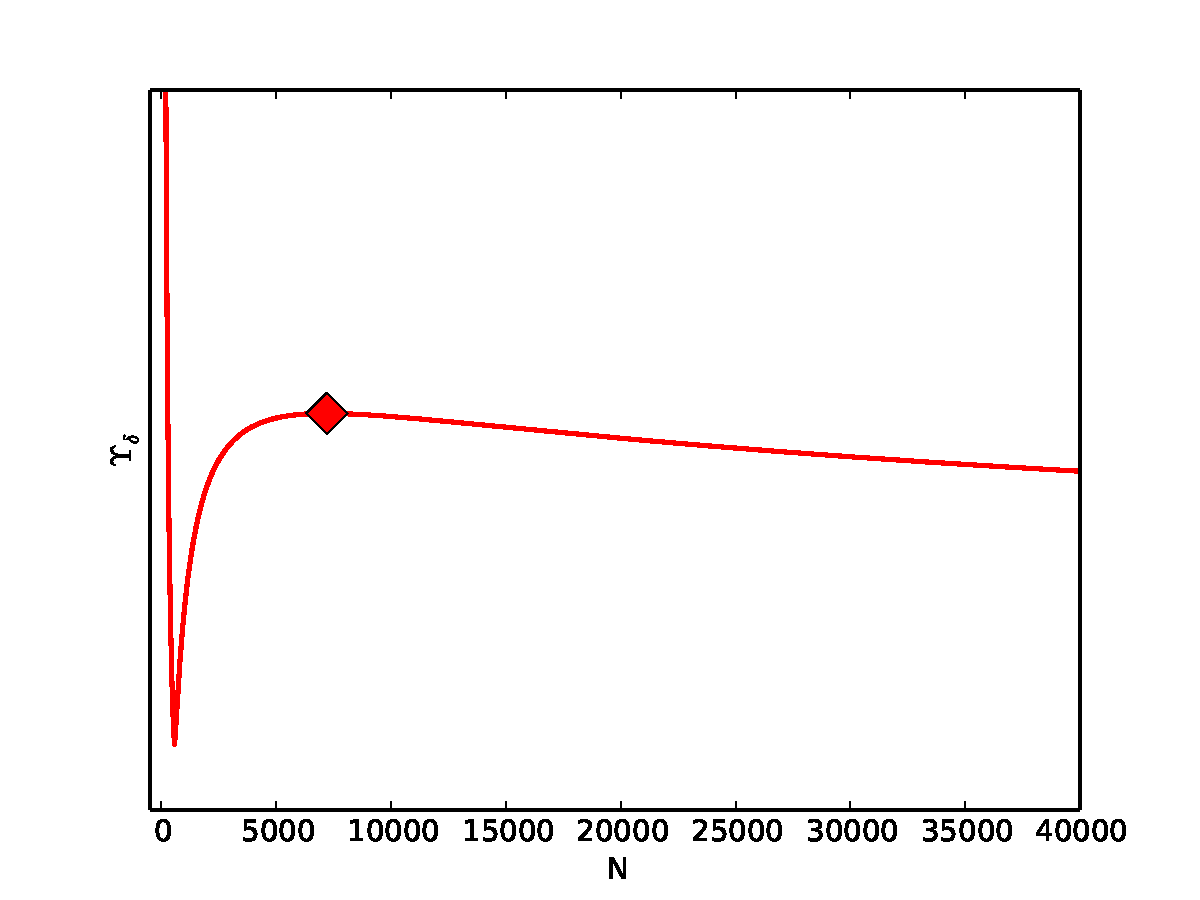
\includegraphics[width = \textwidth,center]{Images/upsilon.pdf}
\caption[Cost function $\Upsilon_\delta$ over batch size $N$.]{Cost function $\Upsilon_\delta$ over batch size $N$. The optimal batch size $N^*$ is marked with a diamond. Batch sizes under the global minimum $N_0$ do not guarantee any performance improvement.}
\label{fig:0}
\end{figure}

The main peculiarity of this result is that the step size is constant, in the sense that its value does not depend on the gradient estimate. This can be explained in terms of a duality between step size and batch size: in other conservative adaptive-step size approaches, such as the one proposed with Theorem \ref{theo:5}, the step size is kept small to counteract policy updates that are too off due to bad gradient estimates. When also the batch size is made adaptive, a sufficient number of sample trajectories can be taken to keep the policy update on track even with a constant-valued step size.
\paragraph{}
We now analyze this approach from a more algorithmic perspective.
As already mentioned, under Assumption \ref{assum:4}, Assumption \ref{assum:3} can be restated as:
\[
	N \geq N_0 \triangleq \frac{d_\delta^2}{\norm[\infty]{\gradApp{\vtheta}}^2},
\]
which is always verified by the proposed $N^*$. This means that the adaptive batch size never allows an estimation error larger than the gradient estimate. This is good news, but it may also lead to very high batch sizes once $\vtheta$ is very close to the optimal parameter. An additional stopping condition may be necessary, and one option is simply to set a maximum allowed batch size.
\paragraph{}
Notice also that the optimal batch size, as defined in Theorem \ref{theo:5}, is referred to the upcoming parameter update. However, the optimal batch size can be employed only for the next update, since trajectory samples need to be collected first. This means that, in any practical implementation, the adaptive batch size that we have defined is always "a learning iteration too late". However, it is reasonable to assume that the conditions that determined the optimal batch size will not vary significantly between a learning iteration and the following one. While we need to rely on $N$'s predictive power, we can keep the step size synchronized as follows: compute $\Lambda^*$ as in Corollary \ref{cor:3}, using:
\[
	\epsilon = \frac{d_\delta}{\sqrt{N}},
\]
where $d_\delta$ is computed with the latest available data and $N$ is the batch size used to collect them. A collateral effect of this approach is that, due to integer approximation, the step size is no longer constant. However, the variations in its value should be quite small.
\paragraph{}
These expedients lead to the following algorithm: 
\begin{algorithm}[H]
\caption{Adaptive Policy Gradient}
\label{alg:adabatch}
\begin{algorithmic}
\State set initial policy parametrization $\vtheta$
\State set initial batch size $N$ and maximum batch size $\overline{N}$
\State $c \gets 		\frac{RM_{\phi}^2}{(1-\gamma)^2\sigma^2}\left(\frac{|\mathcal{A}|}{\sqrt{2\pi}\sigma} +	\frac{\gamma}{2(1-\gamma)}\right)$
\State $\epsilon \gets 0$
\While{$\epsilon < |\gradApp{\vtheta}|$} 
\State perform $N$ trajectories following policy 
	$\pi_{\vtheta} \sim \mathcal{N}(\vtheta^T\vphi(s),\sigma)$
\State compute policy gradient estimate $\gradApp{\vtheta}$
\State $k \gets \arg\max_i|\gradApp{\theta_i}|$
\State compute $d_\delta$ with a proper concentration bound
\State $\epsilon \gets \nicefrac{d_\delta}{\sqrt{N}}$
\State $\alpha \gets \frac{
		\left(\norm[\infty]{\gradApp{\vtheta}} - \epsilon\right)^2}
		{2c
		\left(\norm[\infty]{\gradApp{\vtheta}} + \epsilon\right)^2}$
\State $\theta_k \gets \theta_k + \alpha\gradApp{\theta_k}$
\State $N \gets \left\lceil\frac{(13+3\sqrt{17})d_{\delta}^2}{2\norm[\infty]{\gradApp{\vtheta}}^2}\right\rceil$
\State $N \gets \max\{2,\min\{N,\overline{N}\}\}$
\EndWhile
\end{algorithmic}
\end{algorithm}

Notice that there is still a parameter that must be selected by an expert: $\delta$. This is the probability of having a worsening update, since monotonic improvement is guaranteed with probability $(1-\delta)^m$. Intuitively, the choice of $\delta$ depends on risk attitude and should be small in critical applications. However, numerical simulations (see Section \ref{sec:simul}) show that, at least for simple problems, $\delta$ can be set to very high values ($\sim 1$) without compromising monotonic improvement. This can be useful, since larger values of $\delta$ lead to faster convergence.

We now consider some concentration bounds in more detail, providing the values for $d_{\delta}$ and the corresponding explicit expressions for $N^*$.

\subsection{Chebyshev's bound}\label{sec:chebyshev}
We report here the sample mean version of Chebyshev's bound for a generic stochastic variable $X$:
\[
	\Pr(|E[X] - \overline{X}_N| \geq \epsilon) \leq \frac{Var[X]}{N},
\]
where $\overline{X}_N$ is the sample mean over $N$ samples.
In our case we have:
\[
	\delta = \Pr(|\gradJ{\theta_i} - \gradApp{\theta_i}| 
		\geq \epsilon) \leq \frac{Var[\gradApp{\theta_i}]}{N}.
\]
This bound is compliant with Assumption \ref{assum:4} and gives the following expression for $d_\delta$:
\[
d_\delta = \sqrt{\frac{Var[\gradSim{\theta_i}]}{\delta}},
\]
where $\gradSim{\theta_i}$ is the policy gradient approximator (from a single sample trajectory).
The main advantage of this bound is that it doesn't make any assumption on the range of the gradient sample.
\paragraph{}
Using results from \cite{DBLP:journals/nn/ZhaoHNS12} as adapted in \cite{NIPS2013_5186}, we can give explicit formulations for the optimal batch size.
When the REINFORCE \cite{Williams1992} gradient estimator ($\gradRF{\vtheta}$) is used to estimate the gradient, we can use Lemma 5.4 from \cite{NIPS2013_5186} to bound the estimation error as:

\[
\epsilon \leq \frac{1}{\sqrt{N}}\left(\frac{RM_{\phi}(1-\gamma^H)}
				{\sigma(1-\gamma)}\sqrt{\frac{H}{\delta}}\right),
\]

which gives an optimal batch size:
\[
N^* = \frac{(13+3\sqrt{17})R^2M_{\phi}^2H(1-\gamma^H)^2}
	 		{2\delta\sigma^2(1-\gamma)^2
	 			\norm[\infty]{\gradRF{\vtheta}}^2}.
\]
Similarly, when the G(PO)MDP/PGT gradient estimator ($\gradPGT{\vtheta}$) is used, using Lemma 5.5 from \cite{NIPS2013_5186} we have:

\[
\epsilon \leq \frac{1}{\sqrt{N}}\left(\frac{RM_{\phi}}
				{\sigma(1-\gamma)}\sqrt{\frac{1}{\delta}
				\left[\frac{1-\gamma^{2H}}{1-\gamma^2} + H\gamma^{2H} - 2\gamma^H
				\frac{1-\gamma^H}{1-\gamma}\right]}\right)
\]

and

\[
N^* = \frac{(13+3\sqrt{17})R^2M_{\phi}^2
			\left[\frac{1-\gamma^{2H}}{1-\gamma^2} + H\gamma^{2H} - 2\gamma^H
	 		\frac{1-\gamma^H}{1-\gamma}\right]}
	 		{2\delta\sigma^2(1-\gamma)^2
	 			\norm[\infty]{\gradPGT{\vtheta}}^2}.
\]
These results are independent from the baseline used in the gradient estimation. The G(PO)MDP/PGT estimator suffers from a smaller variance if compared with REINFORCE, and the variance bound is indeed tighter.

\subsection{Hoeffding's bound}
We report Hoeffding's bound applied to our case:
\[
	\delta = \Pr(|\gradJ{\theta_i} - \gradApp{\theta_i}| \geq \epsilon)
		 \leq 2e^{-\frac{2\epsilon^2}{N\mathbf{R}^2}},
\]
where $\mathbf{R}$ is the range of the gradient approximator, i.e. $|supp(\gradSim{\theta_i})|$.
This bound is compliant with Assumption \ref{assum:4} and gives:
\[
d_\delta = \mathbf{R}\sqrt{\frac{\log{2/\delta}}{2}},
\]
For the class of policies we are considering, i.e. Gaussian with mean linear in the features, the range can be upper bounded under some assumptions:

\begin{restatable}{lemma}{secondlemma}
For any Gaussian policy $\pi_\theta \sim \mathcal{N}(\vtheta^T\vphi(s),\sigma^2)$, assuming that the action space is bounded ($|a|\leq \overline{A}\:\:\forall a \in \mathcal{A}$) and the policy gradient is estimated on trajectories of length $H$,the range $\mathbf{R}$ of the policy gradient sample $\gradSim{\theta_i}$ can be upper bounded $\forall i=1,\dots,m$ and $\forall \theta$ by
\[
\mathbf{R} \leq \frac{2HM_{\phi}\overline{A}R}{\sigma^2(1-\gamma)}.
\]
\end{restatable}

As we will show in Section \ref{sec:simul}, a more practical solution (even if less rigorous) consists in computing the range as the difference between the largest and the smallest gradient sample seen during learning.

\subsection{Empirical Bernstein's bound}
Tighter concentration bounds allow for smaller batch sizes (which result in more frequent policy updates) and larger step sizes, thus speeding up the learning process and improving long-time average performance. An empirical Bernstein bound from \cite{Mnih:2008:EBS:1390156.1390241} allows to use sample variance instead of the variance bounds from \cite{DBLP:journals/nn/ZhaoHNS12} and to limit the impact of the gradient range. We report the bound for a generic stochastic variable $X$:
\[
	|E[X] - \overline{X}_N| \leq  \sqrt{\frac{2S_N\ln{\nicefrac{3}{\delta}}}{N}}
		+ \frac{3\mathbf{R}\ln{\nicefrac{3}{\delta}}}{N},
\]
where $S_N$ is the sample variance of $X$, defined as:
\[
	S_N = \frac{1}{N}\sum\limits_{i=1}^N(X_i - \overline{X}_N)^2.
\]
Unfortunately, this bound does not satisfy Assumption \ref{assum:4}, giving for the estimation error the following, more complex, expression:
 \[
 \epsilon(N) = \frac{d_\delta}{\sqrt{N}} + \frac{f_\delta}{N},
\]
where
\begin{align*}
d_\delta= \sqrt{2S_N\ln{\nicefrac{3}{\delta}}}, && f=3\mathbf{R}\ln{\nicefrac{3}{\delta}},
\end{align*}

No reasonably simple closed-form solution is available in this case, requiring a linear search of the batch size $N^*$ maximizing $\Upsilon_\delta$. 

The cost function to optimize becomes (already optimized w.r.t the step size):
\[
\Upsilon_{\delta}(\Lambda^*,N) = \frac{\left(\norm[\infty]{\gradApp{\vtheta}} - 
		\sqrt{\frac{2S_N\ln{\nicefrac{3}{\delta}}}{N}} - \frac{3\mathbf{R}\ln{\nicefrac{3}{\delta}}}{N}\right)^4}
		{4cN
		\left(\norm[\infty]{\gradApp{\vtheta}} + 
				\sqrt{\frac{2S_N\ln{\nicefrac{3}{\delta}}}{N}} + \frac{3\mathbf{R}\ln{\nicefrac{3}{\delta}}}{N}\right)^2}.
\]
First of all, Assumption \ref{assum:3} gives the following constraint:
\[
N \geq N_0 := \left(\frac{d_{\delta} + \sqrt{d_{\delta}^2 + 4f_{\delta}\norm[\infty]{\gradApp{\vtheta}}}}
{2\norm[\infty]{\gradApp{\vtheta}}}
\right)^2,
\]
so $N_0$ can be used as the starting point of the linear search.
Computing the derivative w.r.t $N$ we obtain two factors for the numerator:

\begin{align*}
&\left(d_{\delta}\sqrt{N}+f_{\delta} - \norm[\infty]{\gradApp{\vtheta}}N\right)^3, \\
&\left(2d_{\delta}^2N+5d_{\delta}f_{\delta}\sqrt{N}+3d_{\delta}\norm[\infty]{\gradApp{\vtheta}}N^{\nicefrac{3}{2}} +3f_{\delta}^2+6f\norm[\infty]{\gradApp{\vtheta}}N-\norm[\infty]{\gradApp{\vtheta}}^2N^2\right).
\end{align*}
The left first one gives again $N_0$, which is the global minimum. By applying Descartes' rule of signs to the other one, seen as a polynomial in $\sqrt{N}$, we see that it gives just one root. The exact expression of this maximum is too big to be reported and too long to code, but its uniqueness, together with the fact that $\Upsilon_{\delta}$ goes to $0$ as N goes to infinity, justifies the following methodology: to find $N^*$, start from $N_0$ and stop as soon as the value of the cost function $\Upsilon(\Lambda^*,N)$ begins to decrease.
\paragraph{}
Note also that the optimal step size is no longer constant: it can be computed with the expression given in Corollary \ref{cor:3} by setting $\epsilon := \epsilon(N^*)$.
Finally, as for the Hoeffding's bound, the range $\mathbf{R}$ can be upper bounded exactly or estimated from samples.

